\section{Blender exploration team}

During the whole project, this team had two aims. Our first goal was
to discover Blender and Python while other teams focused on the
bibliographical work, to then teach everyone how to use Blender
efficiently and code in Python. Our second goal was to guarantee the
quality of our code by setting up unitary tests and code coverage
tools.

\subsection{Blender discovery}

Blender is written in C++ and Python, but it has a powerful API in
Python, so we did not have to modify the C++ core of Blender. Blender
is also able to show the Python source of its interface, or give the
Python command associated to a manual operation. These features were
really helpful to develop efficiently our programs.


\subsection{Unitary tests}

For each new class we implemented, we also created a unit test
file. The execution was handled by the unitary test library of
Python. We linked our Github repositories with Travis, a website
that runs the unitary test every time a pull request is created.

The advantage of creating these tests is that it forced us to test
deeply our code, and more important, to notice when code modifications
break some other parts of the code. This last feature is really
important for big projects, to avoid creating bugs when modifying the
code.

\subsection{Code coverage}

We also linked our Github repositories with Coveralls, to see what
part of the code was covered by our unitary tests. To ensure a good
coverage, the pull requests had to increase coverage, or they would
automatically be rejected.

\subsection{Code organization}
%% TODO un peu redondant avec "structure of the project" dans intro ? 
This team also organized globally the code of the project. The code of
each plug-in is separated into two parts: one independent from
Blender, containing the \textit{core}, that is, the main algorithms
and data structures. The second part implements the interface with
Blender.


The advantage of this organization is that the first part can be
tested automatically using unit tests. The part using Blender cannot
be tested automatically with Travis, because it needs a lot of
interaction with the graphical interface. Thus, we tried to put
maximum of the complex algorithm in the first part, to allow them to
be tested extensively.

\begin{figure}[h]
  \begin{center}
    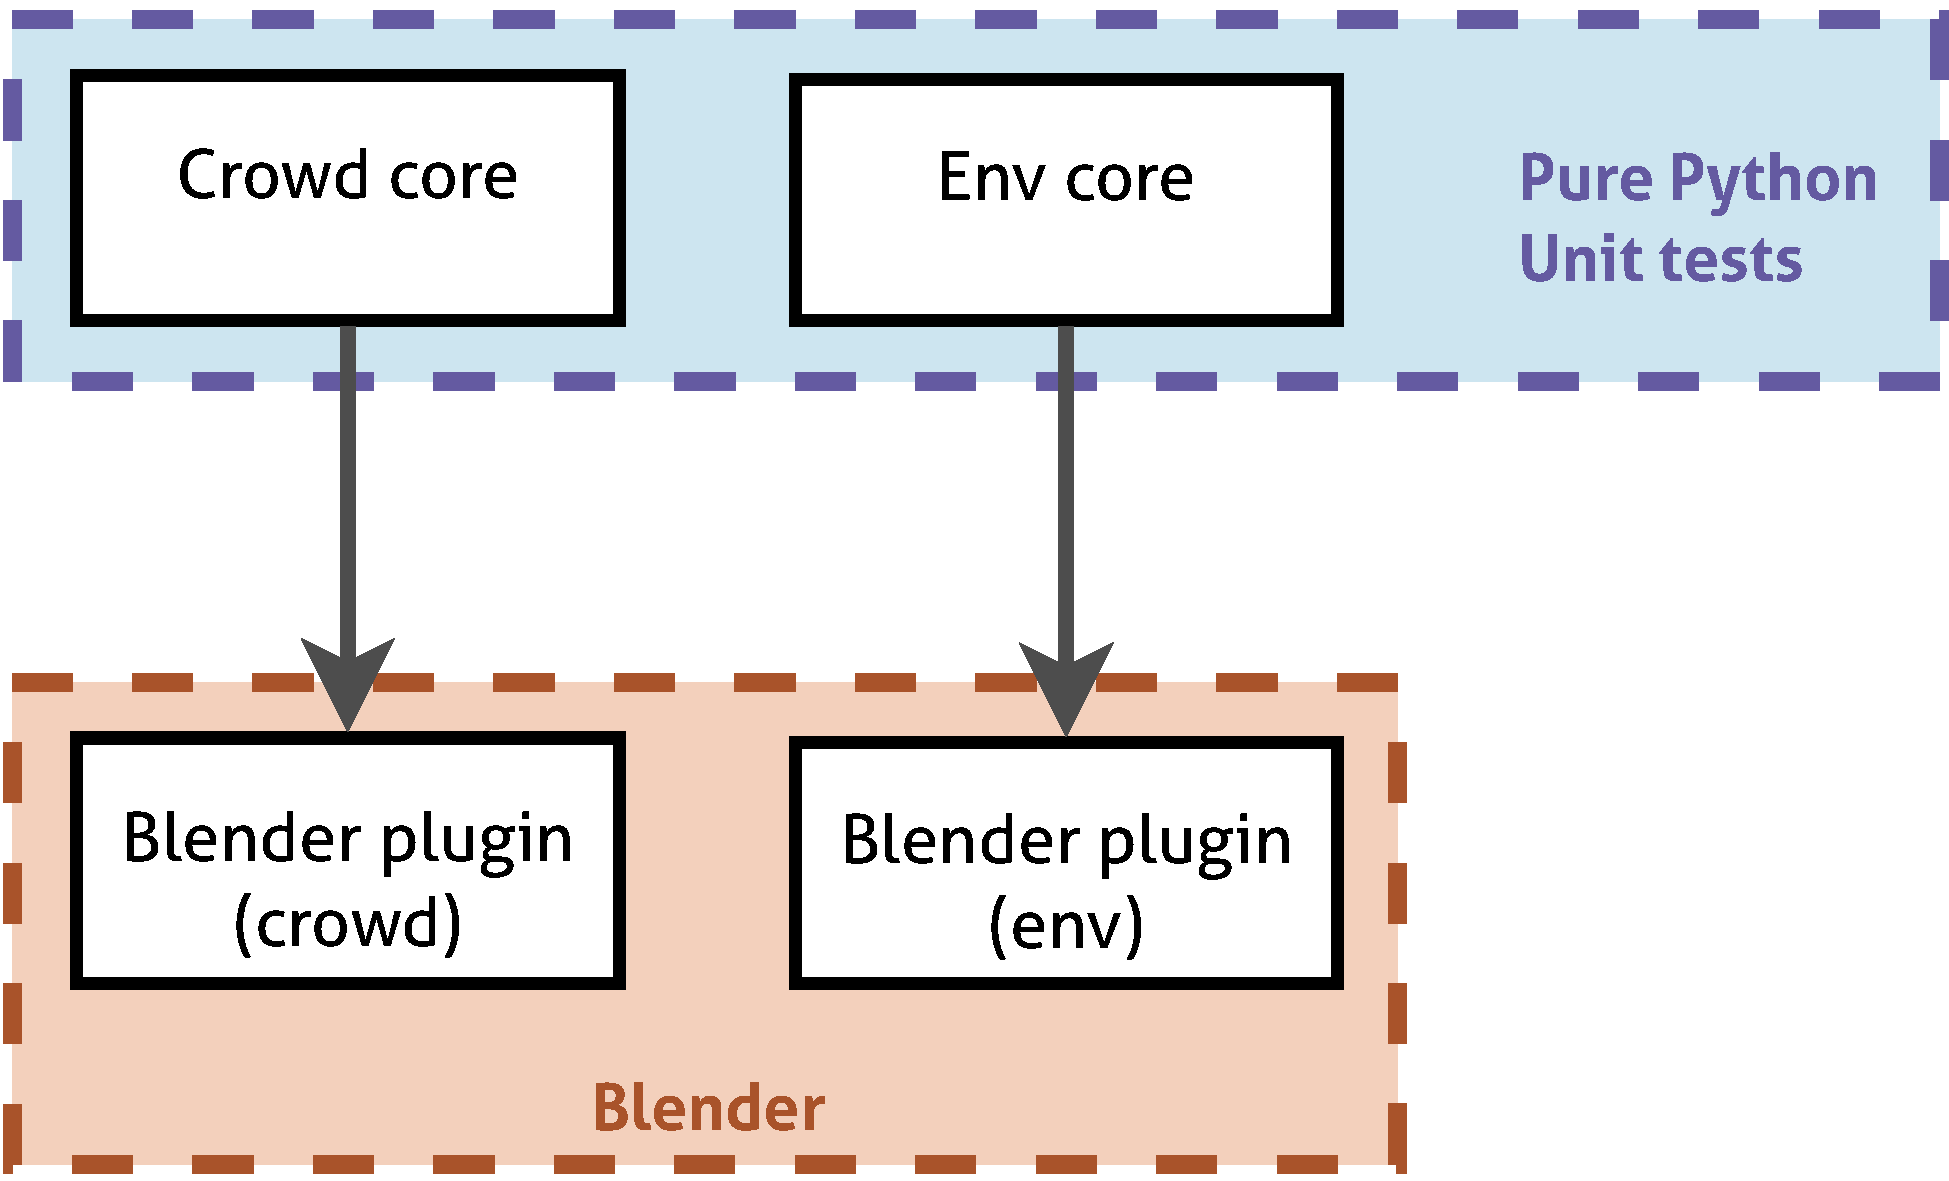
\includegraphics[width=7cm]{img/orga.pdf}
    \caption{Code organization}
    \label{fig:code}
  \end{center}
\end{figure}
